\section{Schemat Metropolisa}

%%%%%%%%%%%%%%%%
	\begin{frame}{Schemat Metropolisa}
		\textbf{Podstawa metody Monte Carlo symulacji molekularnej}
		\begin{figure}
			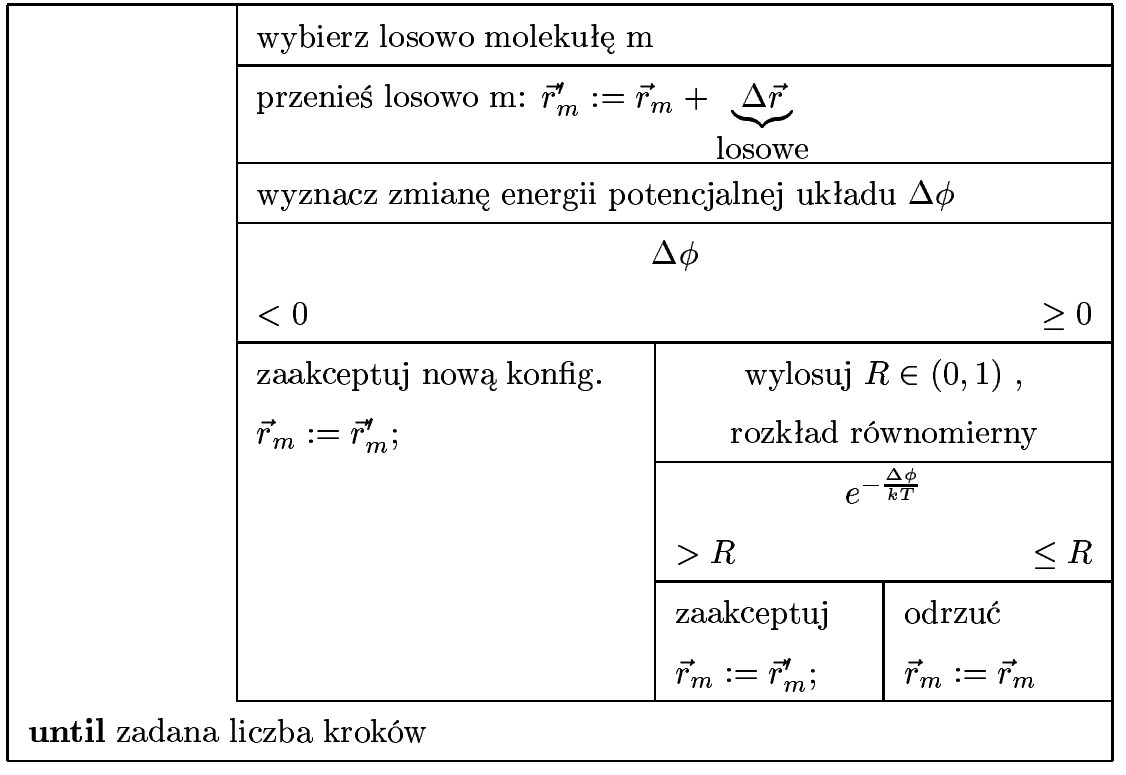
\includegraphics[width=0.67\textwidth]{img/18/metropolis1}
		\end{figure}
		\begin{thebibliography}{9}
			\setbeamertemplate{bibliography item}[article]
			\bibitem{metropolis}{Nicolas Metropolis, Arianna W. Rosenbluth, Marshal M. Rosenbluth, Augusta H. Teller, Edward Teller \newblock J. Chem. Phys. 21 (1953) 1087}
		\end{thebibliography}
	\end{frame}

%%%%%%%%%%%%%%%%

	\begin{frame}{Schemat Metropolisa}
		$$
			\Delta \vec{r} = \delta(\vec{i} \cdot a_x + \vec{j} \cdot a_y  + \vec{k} \cdot a_z)
		$$		
		
		$$
		\delta \text{ - wybrane z góry} \approx 10^{-11}m
		$$		
		
		$$
		a_i \in (-1, 1), Unif
		$$
		
		\begin{figure}
			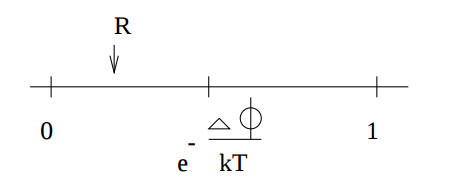
\includegraphics[width=0.5\textwidth]{img/18/metropolis2}
		\end{figure}
		$a_i$, R - liczby pseudolosowe
		
		$\Delta\phi$ - zmiana energii potencjalnej układu w wyniku przesunięcia molekuły m
		
		%Dead link
		%Aplet metropolis/metropolis.html 
	\end{frame}

%%%%%%%%%%%%%%%%
	
	\begin{frame}{Charakterystyka schematu Metropolisa}
		\begin{itemize}
			\item $T \nearrow$ - łatwiej akceptowalne kroki z $H \nearrow (E)$ \\ $ \Rightarrow$ możliwość opuszczenia stanu metastabilnego (lokalnego minimum).
			\item zmiany $H \searrow$ są akceptowane zawsze
		\end{itemize}
		
		Po wielu krokach system $\rightarrow$ stan równowagi termodynamicznej z parametrami oscylującymi wokół wartości średnich zgodnie z rozkładem Boltzmanna
	\end{frame}

\subsection{Łańcuch Markowa}
%%%%%%%%%%%%%%%%
	
	\begin{frame}{Schemat Metropolisa $\rightarrow$ łańcuch Markowa}
		\begin{figure}
				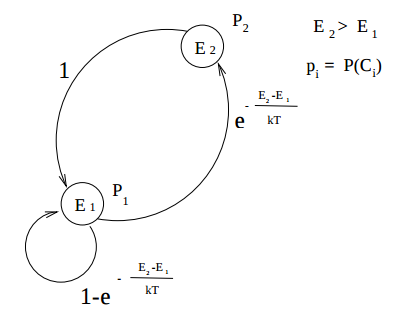
\includegraphics[width=0.5\textwidth]{img/18/markow}
		\end{figure}
		\begin{block}{Zasada równowagi szczegółówej\\ 
		(detailed balance, microscopic reversibility)}
			$$
			p_2 \cdot 1 = p_1 \cdot e^{- \dfrac{E_2 - E_1}{kT}}
			$$
		\end{block}
	\end{frame}

%%%%%%%%%%%%%%%%
	\begin{frame}{Łańcuch Markowa}
		$$
	 	\frac{p1}{p2} = \dfrac{e^{-\frac{E_1}{kT}}}{e^{-\frac{E_2}{kT}}} \rightarrow p_i \sim \underbrace{e^{-\frac{E_i}{kT}}}_{\text{czynnik prawdop. Boltzmanna}}
		$$		
		
		$$
		P(c_i) \sim e^{-\frac{E_i}{kT}}
		$$
		
		$\Rightarrow$ importance sampling: konfiguracje generowane nie losowo - ale z zadanym rozkładem (50-70 \% akceptowanych)
		%Dead link
		%	Notatka nt. niejednorodnych łańcuchów Markowa w SA, dużo bibliografii
		
		% whaaaat
		% http://www.pz.zgora.pl/discuss/al15_2/a6.htm
		
	\end{frame}
	
\section{Uwagi praktyczne}
%%%%%%%%%%%%%%%%
	\begin{frame}{Uwagi praktyczne}
		\textbf{Duże $\Delta\vec{r}$:}
		\begin{itemize}
			\item niski poziom akceptacji
			\item szybsze próbkowanie przestrzeni konfiguracyjnej
		\end{itemize}
		
		\textbf{Dla potencjałów parowych, krótkozasięgowych:}
		\begin{itemize}
			\item przesuwamy tylko 1 cząstkę
			\item dla określenia $\Delta\phi$ - tylko najbliżsi sąsiedzi
		\end{itemize}
		
		\textbf{W przypadku cieczy:}
		\begin{itemize}
			\item każda cząsteczka $\approx 10^3$ przemieszczeń
			\item w modelu $\approx 10^3$ cząsteczek
		\end{itemize}	
		
		\textbf{Force-biased displacement:}
		\begin{itemize}
			\item wszystkie cząsteczki przesuwane równocześnie przeciwnie do gradientu potencjału
		\end{itemize}
		
	\end{frame}
